\section{Memory Management}

\mult{2}

\begin{definition}{Memory Management Introduction}\\
    Critical system resource managed by the OS:
    \begin{itemize}
        \item The Memory Manager controls \\ main memory allocation and usage
        \item Secondary memory: buffer zone (swap)
    \end{itemize}
    
    Memory is organized in a hierarchy:
    \begin{itemize}
        \item Fast cache in 1-3 layers (L1, L2, L3)
        \item Main memory (RAM) - slower but larger
        \item Secondary memory (hard disks, SSDs) \\ - for programs and files
        \item Tertiary memory (backup storage, tapes)
    \end{itemize}
\end{definition}

\begin{concept}{Memory Management Tasks}\\
    OSs handle several memory management tasks:
    \begin{itemize}
        \item Determine how much memory processes require
        \item Deciding where in memory processes are located (position of residency)
        \item Managing how long processes remain in memory (length of residency)
        \item Subdividing memory for co-existence of \\ multiple processes
        \item Handling memory fragmentation
    \end{itemize}
\end{concept}

\multend

\subsubsection{Memory Allocation Approaches}

\mult{2}

\begin{definition}{Free Space Management}\\
    Finding free space during allocation requires efficient algorithms:
    \begin{itemize}
        \item \textbf{Bitmap approach}:
            \begin{itemize}
                \item Space-efficient representation
                \item One bit per allocation unit
                \item Fast free-space finding
            \end{itemize}
        \item \textbf{Linked list approach}:
            \begin{itemize}
                \item List of free blocks
                \item Supports various placement algorithms (first/next/best fit)
            \end{itemize}
    \end{itemize}
\end{definition}

\begin{formula}{Swapping} Free Space Management:
    \begin{itemize}
        \item Secondary memory: temp. storage for processes
        \item When processes are suspended or exit, their memory is freed
        \item When processes restart, they are reloaded into memory
        \item Allows more processes to run concurrently than physical memory would permit
    \end{itemize}
\end{formula}

\multend

\mult{2}

\begin{KR}{Free Space Management}
    \paragraph{Free space management methods}
    \begin{itemize}
        \item Bitmap: Good for uniform access, fixed size
        \item Linked list: Simple but slow random access
        \item Grouping: Combines free blocks into groups
        \item Counting: Stores (address, count) pairs
    \end{itemize}
    
    \paragraph{Evaluation criteria}
    \begin{itemize}
        \item Space efficiency
        \item Access speed
        \item Implementation complexity
        \item Fragmentation handling
        \item Main memory requirements
    \end{itemize}
\end{KR}

\begin{example2}{File System Free Space Management}
    Describe two efficient methods for tracking free blocks:
    
    \textbf{Method 1: Bitmap}
    \begin{itemize}
        \item Each bit represents one block
        \item 0 = free, 1 = allocated (or vice versa)
        \item Fast scanning for free blocks
        \item Compact representation
        \item Requires main memory for efficiency
    \end{itemize}
    
    \textbf{Method 2: Free block list with (start, length) tuples}
    \begin{itemize}
        \item List of contiguous free block ranges
        \item Each entry: (starting block, number of blocks)
        \item Efficient for large contiguous areas
        \item Dynamic size based on fragmentation
    \end{itemize}
\end{example2}

\multend

\raggedcolumns
\columnbreak

\mult{2}

\begin{definition}{Memory Division and Fragmentation}
    \begin{itemize}
        \item \textbf{Static memory division}:
            \begin{itemize}
                \item Memory divided into fixed-size segments
                \item Problem: Internal fragmentation \\ (wasted space within allocated segments)
            \end{itemize}
        \item \textbf{Dynamic memory division}:
            \begin{itemize}
                \item Memory divided according to process needs
                \item Problem: External fragmentation \\ (free space becomes fragmented)
                \item Solution: Compaction (expensive operation)
            \end{itemize}
    \end{itemize}
\end{definition}


\begin{formula}{Buddy Algorithm} Division/Fragmentation:
    \begin{itemize}
        \item Memory divided into blocks of power-of-2 sizes
        \item When a request arrives, the system:
            \begin{itemize}
                \item Finds the smallest block that fits the request
                \item If no suitable block exists, splits a larger block into two 'buddies'
                \item Allocates one buddy and keeps the other free
            \end{itemize}
        \item When a block is freed, the system:
            \begin{itemize}
                \item Checks if its buddy is also free
                \item If both are free, merge into a larger block
                \item Continues merging recursively if possible
            \end{itemize}
        \item Simpler to implement than other DAC
        \item Still experiences some internal fragmentation
    \end{itemize}
\end{formula}



\multend

\begin{KR}{Buddy System Fragmentation}
    \paragraph{Determine buddy block sizes}
    \begin{itemize}
        \item For each allocation request, find smallest power-of-2 block that fits
        \item Block size = $2^{\lceil \log_2(\text{request size}) \rceil}$
    \end{itemize}
   
    \paragraph{Calculate internal fragmentation}
    \begin{itemize}
        \item Fragmentation per block = Block size - Requested size
        \item Total fragmentation \\ = Sum of all individual fragmentations
    \end{itemize}   

    \paragraph{Account for merging}
    \begin{itemize}
        \item When blocks are freed, buddies may merge
        \item Track which blocks remain allocated vs. freed
    \end{itemize}
\end{KR}



\begin{example2}{Buddy System}\\
    Ein Betriebssystem-Kernel verwaltet seine Datenbuffer mit einem Buddy System, wobei insgesamt 8MByte Speicher zur Verfügung stehen. Zur Zeit sind folgende Buffer mit 62KByte, 34KByte und 9KByte alloziert worden. Wie viel Speicher geht dabei durch interne Fragmentierung insgesamt verloren, Angabe in KByte:
    \vspace{2mm}\\
    \begin{minipage}{0.5\linewidth}
    \textbf{Buddy System alloziert in Potenzen von 2:}    
    \begin{itemize}
        \item 62 KByte $\rightarrow$ nächste 2er-Potenz: 64 KByte
        \item 34 KByte $\rightarrow$ nächste 2er-Potenz: 64 KByte  
        \item 9 KByte $\rightarrow$ nächste 2er-Potenz: 16 KByte
    \end{itemize}
    \end{minipage}
    \begin{minipage}{0.5\linewidth}
    \textbf{Interne Fragmentierung = Alloziert - Angefordert:}
    \begin{itemize}
        \item (64 - 62) = 2 KByte
        \item (64 - 34) = 30 KByte
        \item (16 - 9) = 7 KByte
    \end{itemize}
    \end{minipage}
    \vspace{2mm}\\
    Gesamt: 2 + 30 + 7 = \textbf{39 KByte} interne Fragmentierung
\end{example2}

\begin{example2}{Buddy System Analysis}
    8MB system allocates buffers: 62KB, 34KB, 9KB
    
    \textbf{Allocation analysis:}
    \begin{itemize}
        \item \textcolor{orange}{62KB} $\rightarrow$ 64KB block (internal fragmentation: 2KB)
        \item \textcolor{blue}{34KB} $\rightarrow$ 64KB block (internal fragmentation: 30KB)
        \item \textcolor{frog}{9KB} $\rightarrow$ 16KB block (internal fragmentation: 7KB)
        \item Total internal fragmentation: 2 + 30 + 7 = 39KB
    \end{itemize}

    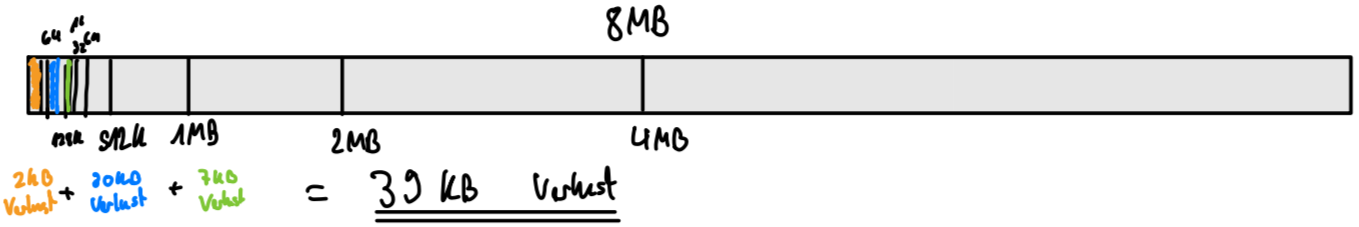
\includegraphics[width=\linewidth]{BUDDYSYSTEM_SEP19.png}
    
    The remaining memory is still available for allocation but in specific block sizes according to the buddy system structure.
\end{example2}





\columnbreak

\subsection{Virtual Memory}



\begin{definition}{Virtual Memory}\\
    Leverages program behavior characteristics:
    \begin{itemize}
        \item Programs exhibit spatial locality (tend to use a limited area of code at any time)
        \item Entire processes don't need to be fully resident in memory
        \item Non-required code/data can be swapped out when not immediately needed
        \item Enables more processes to run concurrently
        \item Must be transparent to programmer/process
    \end{itemize}
\end{definition}

\mult{2}

\begin{theorem}{Translation Lookaside Buffer (TLB)}\\
    The TLB addresses the performance overhead of \\ page table lookups:
    \begin{itemize}
        \item Cache for recently accessed page table entries
        \item Small (typically ~64 entries)
        \item Uses content-addressable memory (CAM) for fast lookups
        \item Memory access process with TLB:
            \begin{itemize}
                \item Check TLB for page number
                \item If found (TLB hit), use frame number directly
                \item If not found (TLB miss), search page table
                \item If not in page table, trigger page fault
                \item Add entry to TLB for future accesses
            \end{itemize}
    \end{itemize}
\end{theorem}

\begin{concept}{Address Translation} logical $\leftrightarrows$ physical\\
    Virtual memory requires translation between logical and pysical addresses:
    \begin{itemize}
        \item Logical address consists of page-nr. and -offset
        \item Page nr. used to look up frame nr. in page table
        \item Physical address formed by combining frame number with page offset
        \item Translation process:
            \begin{itemize}
                \item Extract page nr. and offset from logical addr.
                \item Use page nr. to index page table
                \item Retrieve frame nr. from page table
                \item Combine frame nr. with offset to form \\ physical address
            \end{itemize}
    \end{itemize}
\end{concept}



\multend

\begin{definition}{Paging} mechanism that enables virtual memory:
    \begin{itemize}
        \item Process memory is divided into fixed-size pages
        \item Physical memory is divided into frames of the same size
        \item Pages are loaded into frames as needed
        \item Memory Management Unit (MMU) manages mapping between pages and frames
        \item Typically uses 'on-demand paging' (lazy loading)
            \begin{itemize}
                \item Only loads pages when they are accessed
                \item Sometimes prefetches additional pages based on locality
            \end{itemize}
        \item Process has set of resident pages in memory
            \begin{itemize}
                \item Resident set: All process pages in memory
                \item Working set: Pages currently being used
            \end{itemize}
    \end{itemize}
\end{definition}

\mult{2}

\begin{theorem}{Page Tables} \\ Maintain mapping between pages and frames:
    \begin{itemize}
        \item Each entry contains a frame number
        \item Entries also include status bits:
            \begin{itemize}
                \item Valid bit: Indicates if page holds valid data
                \item Present bit: Indicates if page is in memory
                \item Modified bit (dirty): Indicates if page has been written to
                \item Referenced bit: Indicates recent usage
                \item Protection bits: Control read/write/execute permissions
            \end{itemize}
        \item Page tables are stored in main memory
        \item Can be very large for large address spaces
    \end{itemize}
\end{theorem}

\begin{concept}{Page Replacement}\\
    $\rightarrow$ when memory is full and a new page is needed
    \begin{itemize}
        \item System must decide which resident page to evict
        \item Can use global strategy (any process's pages) or local strategy (only faulting process's pages)
    \end{itemize}
        Common page replacement algorithms:
            \begin{itemize}
                \item Optimal: Replace page used furthest in future (theoretical only)
                \item Least Recently Used (LRU): \\ Replace page unused for longest time
                \item First-In-First-Out (FIFO): Replace oldest page
            \end{itemize}
\end{concept}


\multend

\begin{KR}{Page Table Calculations}
    \paragraph{Extract address components}
    \begin{itemize}
        \item Page Directory bits determine max number of page tables
        \item Page Number bits determine entries per page table
        \item Offset bits determine page size: $2^{\text{offset bits}}$
    \end{itemize}
    
    \paragraph{Calculate system limits}
    \begin{itemize}
        \item Page size = $2^{\text{offset bits}}$ bytes
        \item Max page tables = $2^{\text{directory bits}}$
        \item Entries per page table = $2^{\text{page number bits}}$
        \item Max frames = Max page tables $\times$ Entries per table
    \end{itemize}
\end{KR}

\begin{example2}{Page Tables}\\
    Ein Prozessor besitzt eine Wortbreite von 32Bit. Pointer (Adressen) werden in 32Bit Worten gespeichert, aber nur die 24 tieferwertigen Bits werden für die Adressbildung verwendet (Bits 25-31sind auf 0 gesetzt).
    
    Die logische Adresse ist wie folgt strukturiert:
    \begin{center}
    \begin{tabular}{|c|c|c|}
    \hline
    6-Bit Page Directory & 8-Bit Page Nummer & 10-Bit Offset \\
    \hline
    \end{tabular}
    \end{center}
    
    a) Wie gross ist eine Page, Angabe in KBytes?\\
    b) Wie viele Bytes enthält das Page Directory, wenn pro Eintrag ein Pointer (Adresse) auf eine Page Tabelle eingetragen wird, Angabe in KBytes?\\
    c) Wie viele Page Tabellen kann ein Prozess maximal haben?\\
    d) Wie viele Frames kann das System maximal haben?
    
    \tcblower

    \textbf{Lösung:}
    
    a) Page-Grösse = 2\textsuperscript{10} Bit = 1024 Bytes = \textbf{1 KByte}
    
    b) Page Directory:
    \begin{itemize}
        \item 6 Bit $\rightarrow$ 2\textsuperscript{6} = 64 Einträge
        \item 4 Bytes pro Adresse
        \item 64 × 4 = 256 Bytes = \textbf{0.25 KBytes}
    \end{itemize}
    
    c) Page Tabellen: 6 Bit $\rightarrow$ 2\textsuperscript{6} = \textbf{64 Page Tabellen}
    
    d) Frames im System:
    \begin{itemize}
        \item 24 Bit physische Adresse
        \item 10 Bit Offset pro Frame
        \item Frame-Bits: 24 - 10 = 14 Bit
        \item Maximale Frames: 2\textsuperscript{14} = \textbf{16384 Frames}
    \end{itemize}

\end{example2}

\raggedcolumns
\columnbreak

\subsection{Page Replacement}

\begin{concept}{Page Replacement Algorithms}
    \paragraph{Least Recently Used (LRU)}
    \begin{itemize}
        \item Ersetze die Page, die am längsten nicht verwendet wurde
        \item Gute Performance, aber aufwändig zu implementieren
        \item Benötigt Zeitstempel oder Zugriffs-Historie
        \item Approximation durch Clock Algorithm oder Second Chance
    \end{itemize}
    
    \paragraph{First-In-First-Out (FIFO)}
    \begin{itemize}
        \item Ersetze die älteste Page (first loaded)
        \item Einfach zu implementieren mit Queue
        \item Kann zu Belady's Anomaly führen
        \item Nicht optimal, da alte Pages oft noch verwendet werden
    \end{itemize}
    
    \paragraph{Optimal (OPT)}
    \begin{itemize}
        \item Ersetze Page, die am spätesten wieder verwendet wird
        \item Theoretisch optimal, praktisch nicht implementierbar
        \item Benötigt Zukunftswissen über Page-Zugriffe
        \item Wird als Benchmark für andere Algorithmen verwendet
    \end{itemize}
    
    \paragraph{Implementation Tips}
    \begin{itemize}
        \item Page Fault tritt auf bei erstem Zugriff auf neü Page
        \item Bei mehreren Kandidaten: Wähle Frame mit kleinster Nummer
        \item Clock Algorithm: Circular list mit Reference Bit
        \item Working Set: Berücksichtige lokale vs. globale Ersetzung
    \end{itemize}
\end{concept}

\begin{KR}{Page Replacement Analysis}
    \paragraph{Algorithm comparison factors}
    \begin{itemize}
        \item Page fault frequency
        \item Implementation complexity
        \item Hardware support requirements
        \item Performance under different workloads
        \item Memory overhead for bookkeeping
    \end{itemize}
    
    \paragraph{Common algorithms}
    \begin{itemize}
        \item FIFO: Simple, poor performance
        \item LRU: Good performance, moderate complexity
        \item Clock: Approximates LRU, hardware efficient
        \item Optimal: Theoretical best, not implementable
    \end{itemize}
\end{KR}

\begin{example2}{Page Replacement Algorithms}
    Compare LRU and FIFO page replacement algorithms:
    
    \textbf{LRU (Least Recently Used) typically causes fewer page faults because:}
    \begin{itemize}
        \item Exploits locality principle
        \item Recently accessed pages likely to be accessed again soon
        \item Keeps "hot" pages in memory longer
        \item Better prediction of future access patterns
    \end{itemize}
    
    \textbf{FIFO (First In, First Out):}
    \begin{itemize}
        \item Simple implementation
        \item No consideration of access patterns
        \item May replace frequently used pages
        \item Can suffer from Belady's anomaly
    \end{itemize}
    
    \textbf{Optimal algorithm (theoretical):}
    \begin{itemize}
        \item Replace page that will be accessed furthest in future
        \item Not implementable (requires future knowledge)
        \item Used as performance benchmark
    \end{itemize}
\end{example2}

\begin{KR}{LRU Page Replacement}
    \paragraph{Track page access order}
    \begin{itemize}
        \item Maintain timestamp or access order for each page in memory
        \item On page fault, identify least recently used page
        \item Replace LRU page with new page
    \end{itemize}
    
    \paragraph{Handle page faults}
    \begin{itemize}
        \item Mark page fault when referenced page not in memory
        \item Load new page into frame of LRU page
        \item Update access timestamps for all affected pages
    \end{itemize}
    
    \paragraph{Apply demand paging}
    \begin{itemize}
        \item First access to any page is compulsory miss
        \item Subsequent accesses depend on memory capacity and access pattern
    \end{itemize}
\end{KR}

\begin{example2}{Least Recently Used (LRU)}\\
    Ein Prozess referenziert der Reihe nach folgende Pages:
    \begin{center}
    8 7 5 8 7 3 5 1 3 4 2 1 8 3 1 2
    \end{center}
    
    Gehen Sie davon aus, dass zu Beginn keine Pages im Speicher stehen und dass auch das erstmalige Laden einer Page als Page Fault gezählt wird (demand paging). Pro Prozess stehen 4 Frames zur Verfügung.
    
    Tragen Sie in unten stehender Tabelle die den Frames zugewiesenen Pages für den Least Recently Used Algorithmus. Das Page mit diesem Zugriff am weitesten zurückliegend wird dann mit ein neüs Page ersetzt.
    
    Markieren Sie die Spalten mit einem Stern, wo ein Page Fault auftritt. Nehmen Sie an, dass ausschliesslich Demand Paging verwendet wird. Wenn mehrere Frames für das placement resp. replacement in Frage kommen, muss der Frame mit der kleinsten Nummer gewählt werden.
    
    \tcblower
    
    \textbf{Lösung:}
    
    \begin{center}
    \begin{tabular}{|l|c|c|c|c|c|c|c|c|c|c|c|c|c|c|c|c|}
    \hline
    Referenzen & 8 & 7 & 5 & 8 & 7 & 3 & 5 & 1 & 3 & 4 & 2 & 1 & 8 & 3 & 1 & 2 \\
    \hline
    frame 1 & 8* & 8 & 8 & 8 & 8 & 8 & 8 & 1* & 1 & 1 & 1 & 1 & 1 & 1 & 1 & 1 \\
    \hline
    frame 2 & & 7* & 7 & 7 & 7 & 7 & 7 & 7 & 7 & 4* & 4 & 4 & 8* & 8 & 8 & 8 \\
    \hline
    frame 3 & & & 5* & 5 & 5 & 5 & 5 & 5 & 5 & 5 & 2* & 2 & 2 & 2 & 2 & 2 \\
    \hline
    frame 4 & & & & & & 3* & 3 & 3 & 3 & 3 & 3 & 3 & 3 & 3 & 3 & 3 \\
    \hline
    page fault & × & × & × & & & × & & × & & × & × & & × & & & \\
    \hline
    \end{tabular}
    \end{center}
    
    \textbf{Page Faults:} 8 von 16 Zugriffen\\
    Compulsory Page Faults: die ersten 4 (8, 7, 5, 3) sind unvermeidlich, da die Pages noch nicht im Speicher sind.\\
    
    \textbf{LRU-Logik:}
    \begin{itemize}
        \item Bei jedem Zugriff wird die "letzte Verwendung" der Page aktualisiert
        \item Bei einem Page Fault wird die am längsten nicht verwendete Page ersetzt
        \item Zeitstempel oder Zugriffs-Historie bestimmen LRU-Page
    \end{itemize}
    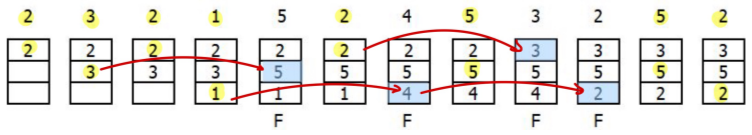
\includegraphics[width=0.8\linewidth]{page_replacement_SEP19.png}
\end{example2}





\subsection{Virtual Memory Addressing}

\begin{KR}{Virtual Memory Address Analysis}
    \paragraph{Address structure calculation}
    \begin{itemize}
        \item Page offset bits = $log_2$(page size in bytes)
        \item Remaining bits = total address bits - offset bits
        \item Bits per level = remaining bits ÷ number of levels
    \end{itemize}
    
    \paragraph{Page table size calculation}
    \begin{itemize}
        \item Entries per table = 2\textsuperscript{bits per level}
        \item Table size = entries × entry size in bytes
        \item Number of tables per level = cumulative from higher levels
    \end{itemize}
    
    \paragraph{Common mistakes to avoid}
    \begin{itemize}
        \item Forgetting to account for page offset bits
        \item Mixing up table levels in size calculations
        \item Not considering that tables should fit in pages
    \end{itemize}
\end{KR}

\begin{example2}{Virtual Memory Address Translation}
    Given: 16KB page size, 47-bit virtual addresses, 3-level paging, 8-byte page table entries.
    
    How is a virtual address structured?
    
    \tcblower
    
    \textbf{Calculation:}
    \begin{itemize}
        \item Page size: 16KB = 2\textsuperscript{14} bytes $\rightarrow$ 14 bits for page offset
        \item Remaining bits: 47 - 14 = 33 bits for page table indexing
        \item 3 levels: 33 ÷ 3 = 11 bits per page table level
    \end{itemize}
    
    \textbf{Address structure:}
    \begin{tabular}{|c|c|c|c|}
        \hline
        Bits 46-36 & Bits 35-25 & Bits 24-14 & Bits 13-0 \\
        \hline
        Level 1 (11 bit) & Level 2 (11 bit) & Level 3 (11 bit) & Offset (14 bit) \\
        \hline
    \end{tabular}
    
    \textbf{Page table sizes:}
    \begin{itemize}
        \item Level 1: 1 table with 2\textsuperscript{11} = 2048 entries
        \item Level 2: 2048 tables with 2048 entries each
        \item Level 3: 2048\textsuperscript{2} = 4,194,304 tables with 2048 entries each
        \item Each table: 2048 × 8 bytes = 16KB (exactly one page)
    \end{itemize}
\end{example2}

\important{ADD EXERCISE 12 SEP07 SEGMENTATION}

\raggedcolumns
\pagebreak

\subsection{Memory Management Analysis}

\mult{2}

\begin{formula}{Buddy System}
    \begin{itemize}
        \item Alloziert in Potenzen von 2 (1, 2, 4, 8, 16, ... KByte)
        \item Interne Fragmentierung = Alloziert - Angefordert
        \item Nächste grössere 2er-Potenz finden: 2\textsuperscript{n} $\geq$ Anforderung
        \item Beispiel: 33 KByte $\rightarrow$ 64 KByte (2\textsuperscript{6})
    \end{itemize}
\end{formula}

\begin{formula}{Page Table Berechnung}
    \begin{itemize}
        \item Page-Grösse = 2\textsuperscript{Offset-Bits} Bytes
        \item Anzahl Pages = 2\textsuperscript{Page-Number-Bits}
        \item Page Directory Grösse = 2\textsuperscript{Directory-Bits} × Pointer-Grösse
        \item Maximale Frames = 2\textsuperscript{(Physische-Adress-Bits - Offset-Bits)}
    \end{itemize}
\end{formula}

\begin{formula}{Addressaufteilung}
    \begin{itemize}
        \item Logische Adresse = Page Directory + Page Number + Offset
        \item Physische Adresse = Frame Number + Offset
        \item Page Table Entry enthält Frame Number
        \item Translation: Page Number $\rightarrow$ Frame Number
    \end{itemize}
\end{formula}

\begin{concept}{Memory Hierarchy}
    \begin{itemize}
        \item Page Directory zeigt auf Page Tables
        \item Page Tables zeigen auf Frames
        \item Mehrstufige Page Tables reduzieren Speicherbedarf
        \item TLB cached häufig verwendete Translations
    \end{itemize}
\end{concept}

\multend

\subsubsection{Memory Access Time Calculation}


\begin{KR}{Average Memory Access Time}
    
    \paragraph{Calculation method}
    \begin{itemize}
        \item Start from L1 cache (always accessed first)
        \item Apply formula from innermost level outward
        \item For each miss, calculate probability of accessing next level (e.g. L3 miss probability = $(1-h_1) \times (1-h_2) \times (1-h_3)$)
        \item Multiply access time by probability of reaching that level
        \item Sum all weighted access times
    \end{itemize}
    
    \paragraph{Formula}
    \begin{itemize}
        \item $T_{avg} = T_{L1} + (1-h_1) \times T_{L2} + (1-h_1)(1-h_2) \times T_{L3} + \ldots$
        \item Convert clock cycles to nanoseconds: Time = Cycles $\times$ Clock period (or Cycle time)
        \item Clock period = 1 / Frequency
    \end{itemize}
\end{KR}

\begin{example2}{Memory Access Time Calculation}
    2 GHz processor (0.5 ns cycle), 90\% hit rate on all levels:
    
    \begin{tabular}{|l|l|}
        \hline
        L1 Cache & 4 cycles = 2.0 ns \\
        L2 Cache & 10 cycles = 5.0 ns \\
        L3 Cache & 40 cycles = 20.0 ns \\
        Main Memory & 60 ns \\
        \hline
    \end{tabular}
    
    \tcblower
    
    \textbf{Calculation:}
    \begin{itemize}
        \item L1 access: $4 \times 0.5 = 2$ ns (always accessed)
        \item L2 access: $10 \times 0.5 = 5$ ns (10\% probability)
        \item L3 access: $40 \times 0.5 = 20$ ns (1\% probability)  
        \item Main memory: 60 ns (0.1\% probability)
        \item $T_{avg} = 2 + 0.1 \times 5 + 0.01 \times 20 + 0.001 \times 60$
        \item $T_{avg} = 2 + 0.5 + 0.2 + 0.06 = 2.76$ ns
    \end{itemize}
\end{example2}

\subsubsection{Cache Performance Analysis}

\important{TODO: add theory and example!!}

\begin{KR}{Cache Hit Rate Calculation}
    \paragraph{Problem identification}
    \begin{itemize}
        \item Given: Array access pattern, processor architecture, cache block size
        \item Find: Cache hit rate during sequential array access
    \end{itemize}

    \paragraph{Given information analysis}
    \begin{itemize}
        \item Identify data type size (e.g., int = 4 bytes on 32-bit system)
        \item Note cache line size (e.g., 64 bytes)
        \item Determine access pattern (sequential vs. random)
    \end{itemize}
    
    \paragraph{Solution approach}
    \begin{itemize}
        \item Calculate element (data type) size based on processor architecture
        \item Determine how many array elements fit in one cache line
        \item For sequential access: First access to cache line = miss, rest = hits
    \end{itemize}
    
    \paragraph{Key formulas}
    \begin{itemize}
        \item Elements per cache line = Cache line size / Element size
        \item Hit rate = Number of hits / Total accesses
        \item For 32-bit processor: int = 4 bytes
        \item For 64-bit processor: int = 4 bytes, long = 8 bytes
    \end{itemize}
\end{KR}

\begin{example2}{Cache Access Analysis}
    Given code accessing an integer array sequentially:
    
\begin{lstlisting}[language=C, style=basesmol]
#define N (10*1000*1000)
int arVL[N];
for (int i = 0; i < N; i++) {
    sum += arVL[i];
}
\end{lstlisting}

Calculate hit rate on a 32-bit processor with 64-byte cache lines.

    \tcblower
    
    \textbf{Analysis:}
    \begin{itemize}
        \item 32-bit system (processor): int = 4 bytes
        \item Cache line size: 64 bytes
        \item Elements per cache line: 64/4 = 16 integers
        \item Access pattern: Sequential $\rightarrow$ first access per line: cache miss
        \item For every 16 accesses: 1 miss + 15 hits
        \item Hit rate: $h_c$ = 15/16 = 0.9375 = 93.75\%
    \end{itemize}
\end{example2}

\raggedcolumns
\pagebreak

\subsection{Linux Memory Management}

\mult{2}

\begin{definition}{Linux Page Table Organization}\\
    Linux uses a hierarchical page table structure:
    \begin{itemize}
        \item Multi-level page directory to reduce size and improve lookup speed
        \item Typically 4-level structure:
            \begin{itemize}
                \item Page Global Directory (PGD)
                \item Page Upper Directory (PUD)
                \item Page Middle Directory (PMD)
                \item Page Table Entry (PTE)
            \end{itemize}
        \item Allows efficient handling of sparse address spaces
        \item Only allocates page tables for used parts of address space
    \end{itemize}
\end{definition}

\begin{definition}{Huge Pages} supported to improve performance:
    \begin{itemize}
        \item Standard page size is 4KB
        \item Huge pages can be 2MB or 1GB \\(architecture-dependent)
        \item Advantages:
            \begin{itemize}
                \item Reduces TLB pressure (fewer entries needed to cover same memory)
                \item Improves performance for memory-intensive applications
                \item More efficient for large memory allocations
            \end{itemize}
        \item Uses higher-level page table entries (PUD/PMD)
        \item Requires explicit configuration
    \end{itemize}
\end{definition}

\multend

\begin{concept}{Memory Zones}\\
    Linux divides physical memory into zones to handle hardware limitations:
    \begin{itemize}
        \item \textbf{ZONE\_DMA}: Memory addressable by DMA controllers (typically below 16MB)
        \item \textbf{ZONE\_NORMAL}: Regularly mapped memory in kernel space
        \item \textbf{ZONE\_HIGHMEM}: Memory beyond what the kernel can directly address
        \item Zones are managed separately to accommodate different hardware constraints
        \item Each zone has its own free lists and allocation policies
    \end{itemize}
\end{concept}

\begin{theorem}{Buddy Allocator}
    Linux uses the buddy system for frame allocation:
    \begin{itemize}
        \item Fundamental allocation unit is the page frame
        \item Maintains lists of free blocks of various sizes (powers of 2)
        \item When a process requests memory:
            \begin{itemize}
                \item System finds the smallest block size that fits the request
                \item If necessary, splits larger blocks into "buddies"
                \item Allocates memory from appropriate free list
            \end{itemize}
        \item When memory is freed:
            \begin{itemize}
                \item System checks if buddy is also free
                \item If so, merges buddies to form larger block
                \item Continues merging recursively if possible
            \end{itemize}
        \item Maintains free lists up to MAX\_ORDER-1 (typically 10, so up to 512 contiguous pages)
    \end{itemize}
\end{theorem}

\begin{theorem}{Slab Allocator}
    Linux uses the slab allocator for kernel objects:
    \begin{itemize}
        \item Kernel often requires small allocations for data structures
        \item Pages (4KB) are too large for many kernel objects
        \item Slab allocator:
            \begin{itemize}
                \item Gets pages from buddy allocator
                \item Divides them into smaller objects of specific types
                \item Maintains caches of frequently used object types
                \item Reuses recently freed objects (helps prevent fragmentation)
                \item Preserves object state between uses
            \end{itemize}
        \item Improves memory utilization and allocation speed
        \item Minimizes internal fragmentation
    \end{itemize}
\end{theorem}

\begin{formula}{Memory Compaction}
    Linux performs memory compaction to address fragmentation:
    \begin{itemize}
        \item Problem: Buddy allocator may not find large contiguous blocks
        \item Solution: kcompactd daemon performs compaction
        \item Process:
            \begin{itemize}
                \item Balances memory zones by swapping out non-working-set pages
                \item Moves movable pages toward the top of the memory zone
                \item Leaves bottom of memory free for new allocations
                \item Creates larger contiguous free blocks
            \end{itemize}
        \item Performed on-demand or periodically
        \item Enables allocation of huge pages and other large memory blocks
    \end{itemize}
\end{formula}

\begin{formula}{Shared Libraries}
    Linux uses shared libraries to reduce memory usage:
    \begin{itemize}
        \item Multiple processes can use the same library code
        \item Libraries compiled with -fPIC (Position Independent Code)
        \item Dynamically linked with processes using ld.so
        \item Read-only code pages memory-mapped into processes
        \item Benefits:
            \begin{itemize}
                \item Reduces memory footprint
                \item Shared code/text pages only loaded once
                \item Only data pages need to be process-specific
            \end{itemize}
        \item Challenge: Version compatibility ("DLL hell")
    \end{itemize}
\end{formula}

\begin{formula}{Page Reclamation}
    Linux uses page reclamation to recover memory:
    \begin{itemize}
        \item Working set: Pages actively in use by processes
        \item Resident set: All pages in memory
        \item A page is in the working set if:
            \begin{itemize}
                \item Accessed via process address space
                \item Accessed via system call
                \item Accessed via device driver
            \end{itemize}
        \item Linux identifies non-working set pages using a bitmap
        \item Pages marked idle can be reclaimed when memory is needed
    \end{itemize}
\end{formula}

\begin{formula}{Least Recently Used in Linux}\\
    Linux implements a two-stage LRU algorithm:
    \begin{itemize}
        \item Maintains two lists of page frames:
            \begin{itemize}
                \item Active list: Recently accessed pages
                \item Inactive list: Less recently accessed pages
            \end{itemize}
        \item Pages move between lists based on access patterns
        \item Inactive pages are candidates for reclamation
        \item Recently accessed inactive pages can be promoted to active list
        \item Linux uses a global strategy for page reclamation
        \item Recent development: Multi-Generational LRU (MGLRU)
            \begin{itemize}
                \item Assigns generation numbers to page frames based on recent access
                \item Older generations are reclaimed first
                \item Improves performance and responsiveness
            \end{itemize}
    \end{itemize}
\end{formula}

\begin{theorem}{Out-of-Memory (OOM) Killer}
    Linux has an OOM Killer to handle critical memory shortages:
    \begin{itemize}
        \item Activates when system is critically low on memory
        \item Linux tends to be optimistic in memory allocation
            \begin{itemize}
                \item Processes typically request more memory than needed
                \item System may over-allocate (more than physical memory)
            \end{itemize}
        \item OOM Killer selects processes to terminate based on heuristics
            \begin{itemize}
                \item Considers memory usage, runtime, nice value, etc.
                \item Each process has an oom\_score in /proc/\$PID/oom\_score
                \item Can be adjusted through oom\_score\_adj
            \end{itemize}
        \item Prioritizes system stability over individual process survival
    \end{itemize}
\end{theorem}

\begin{KR}{Memory Management Analysis in Linux}
    \paragraph{Basic memory information}
    \begin{itemize}
        \item Display system memory usage: \texttt{free -h}
        \item View memory details: \texttt{cat /proc/meminfo}
        \item Check process memory usage: \texttt{ps -eo pid,ppid,cmd,vsz,rss}
        \item Interactive memory monitor: \texttt{top} or \texttt{htop}
    \end{itemize}
    
    \paragraph{Process memory analysis}
    \begin{itemize}
        \item Check process memory maps: \texttt{cat /proc/\$PID/maps}
        \item View process memory status: \texttt{cat /proc/\$PID/status}
        \item Analyze memory usage in detail: \texttt{pmap \$PID}
        \item Track memory over time: \texttt{smem}
    \end{itemize}
    
    \paragraph{Memory page information}
    \begin{itemize}
        \item Get page size: \texttt{getconf PAGE\_SIZE}
        \item Check huge pages: \texttt{cat /proc/meminfo | grep Huge}
        \item View page stats: \texttt{cat /proc/pagetypeinfo}
        \item Check page faults: \texttt{ps -o min\_flt,maj\_flt \$PID}
    \end{itemize}
    
    \paragraph{Memory limits and control}
    \begin{itemize}
        \item Set memory limits: \texttt{ulimit -m [size]}
        \item Control cgroup memory: \texttt{echo [value] > /sys/fs/cgroup/memory/[group]/memory.limit\_in\_bytes}
        \item Check swappiness: \texttt{cat /proc/sys/vm/swappiness}
        \item Adjust swappiness: \texttt{sysctl vm.swappiness=[value]}
    \end{itemize}
\end{KR}

\begin{example2}{Analyzing Process Memory}
    Check memory usage details for a process:
    
\begin{lstlisting}[language=bash, style=basesmol]
# Get PID of a process
PID=$(pidof firefox)

# Check virtual and resident memory size
ps -o pid,comm,vsz,rss -p $PID

# Analyze memory map segments
cat /proc/$PID/maps | head -10

# View detailed memory status
grep -E 'VmSize|VmRSS|VmData|VmStk|VmExe' /proc/$PID/status

# Map process address space in detail
pmap -x $PID | head -20

# Check page faults
ps -o min_flt,maj_flt -p $PID
\end{lstlisting}

    \tcblower
    
    \textbf{Explanation of memory terms:}
    \begin{itemize}
        \item \textbf{VSZ (Virtual Size)}: Total virtual memory allocated to process
        \item \textbf{RSS (Resident Set Size)}: Actual physical memory used
        \item \textbf{VmData}: Size of data segment
        \item \textbf{VmStk}: Size of stack
        \item \textbf{VmExe}: Size of text segment
        \item \textbf{min\_flt}: Minor page faults (page in memory but not in process's page table)
        \item \textbf{maj\_flt}: Major page faults (page had to be loaded from disk)
    \end{itemize}
\end{example2}

\begin{example2}{Working with Page Size and Memory Allocation}
    Analyzing page size and memory allocation:
    
\begin{lstlisting}[language=C, style=basesmol]
#include <stdio.h>
#include <stdlib.h>
#include <unistd.h>
#include <sys/mman.h>

int main() {
    // Get process ID
    pid_t pid = getpid();
    printf("Process ID: %d\n", pid);
    
    // Get page size
    int page_size = getpagesize();
    printf("Page size: %d bytes\n", page_size);
    
    // Allocate memory for 10 pages
    size_t size = 10 * page_size;
    char *buffer = malloc(size);
    printf("Allocated %zu bytes (%zu pages)\n", 
           size, size / page_size);
    
    // Check page faults before access
    printf("Check page faults with: ps -o min_flt,maj_flt %d\n", pid);
    printf("Press Enter to continue...\n");
    getchar();
    
    // Access the memory (causes page faults)
    for (int i = 0; i < size; i += page_size) {
        buffer[i] = 1;  // Touch one byte per page
    }
    
    // Check page faults after access
    printf("Check page faults again with: ps -o min_flt,maj_flt %d\n", pid);
    printf("Press Enter to continue...\n");
    getchar();
    
    // Allocate page-aligned memory
    void *aligned_buf = NULL;
    int result = posix_memalign(&aligned_buf, page_size, size);
    if (result == 0) {
        printf("Allocated %zu bytes aligned on page boundary\n", size);
    }
    
    // Free memory
    free(buffer);
    free(aligned_buf);
    
    return 0;
}
\end{lstlisting}

    This example demonstrates:
    \begin{itemize}
        \item Getting the system page size
        \item Allocating memory
        \item Observing page faults due to lazy allocation
        \item Creating page-aligned memory allocations
    \end{itemize}
\end{example2}

